% !TEX TS-program = pdflatex
% !TEX encoding = UTF-8 Unicode

% This is a simple template for a LaTeX document using the "article" class.
% See "book", "report", "letter" for other types of document.

\documentclass[12pt]{article} % use larger type; default would be 10pt

\usepackage[utf8]{inputenc} % set input encoding (not needed with XeLaTeX)

%%% Examples of Article customizations
% These packages are optional, depending whether you want the features they provide.
% See the LaTeX Companion or other references for full information.

%%% PAGE DIMENSIONS
\usepackage{geometry} % to change the page dimensions
\geometry{a4paper} % or letterpaper (US) or a5paper or....
% \geometry{margin=2in} % for example, change the margins to 2 inches all round
% \geometry{landscape} % set up the page for landscape
%   read geometry.pdf for detailed page layout information

\usepackage{graphicx} % support the \includegraphics command and options

% \usepackage[parfill]{parskip} % Activate to begin paragraphs with an empty line rather than an indent

%%% PACKAGES
\usepackage{booktabs} % for much better looking tables
\usepackage{array} % for better arrays (eg matrices) in maths
\usepackage{paralist} % very flexible & customisable lists (eg. enumerate/itemize, etc.)
\usepackage{verbatim} % adds environment for commenting out blocks of text & for better verbatim
\usepackage{subfig} % make it possible to include more than one captioned figure/table in a single float
\usepackage{graphicx}
\usepackage[colorlinks, urlcolor=cyan, citecolor=red]{hyperref}
% These packages are all incorporated in the memoir class to one degree or another...

%%% HEADERS & FOOTERS
\usepackage{fancyhdr} % This should be set AFTER setting up the page geometry
\pagestyle{fancy} % options: empty , plain , fancy
\renewcommand{\headrulewidth}{0pt} % customise the layout...
\lhead{}\chead{}\rhead{}
\lfoot{}\cfoot{\thepage}\rfoot{}

%%% SECTION TITLE APPEARANCE
\usepackage{sectsty}

\usepackage{enumitem}

%%% ToC (table of contents) APPEARANCE
\usepackage[nottoc,notlof,notlot]{tocbibind} % Put the bibliography in the ToC
\usepackage[titles,subfigure]{tocloft} % Alter the style of the Table of Contents
\usepackage{dirtree}
\usepackage{authblk}
\renewcommand{\cftsecfont}{\rmfamily\mdseries\upshape}
\renewcommand{\cftsecpagefont}{\rmfamily\mdseries\upshape} % No bold!

%%% END Article customizations

%%% The "real" document content comes below...

\title{OCR Handwriting Project Special Report}
\author{Matthew Mulhall}
\affil{matthew.l.mulhall@uconn.edu}
\begin{document}
\maketitle

\begin{enumerate}[label = (\roman*)]
\item Today's tests were run in order to decide the future of the project as far as trajectory. After several tests I think that it is clear that our data set must be increased. If I had to give an estimation I would say that to realistically solve this problem at high sucess rates, we would need something on the order or 3-5x more images per sample. I believe this is due to the inter-class noise that our model is picking up. It is having a hard time deciding between certain letters because their characteristics are not defined different enough through the data. That being said we still have great success rates given the reality of this problem. For example, our 19 class test currently runs around 80\% accurate. To put this into perspective, it is still 15.2 times better than random guessing. To me, this means our model is built correctly, yet it still doesn't have enough data to properly discern classes. Below I have shown the conclusions of the tests to support my hypothesis.
\item 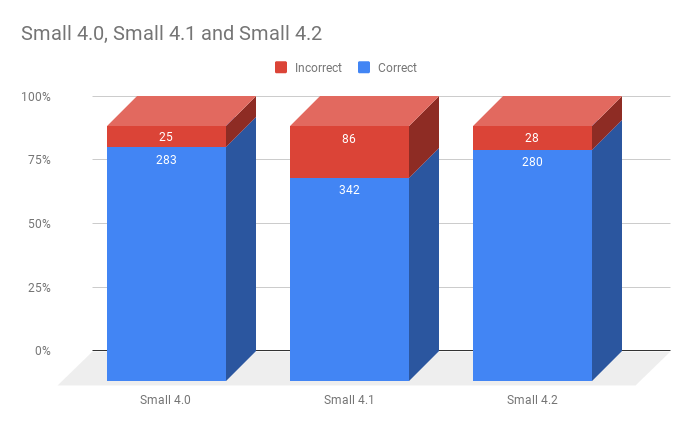
\includegraphics[scale=.7]{charts/overall}
\item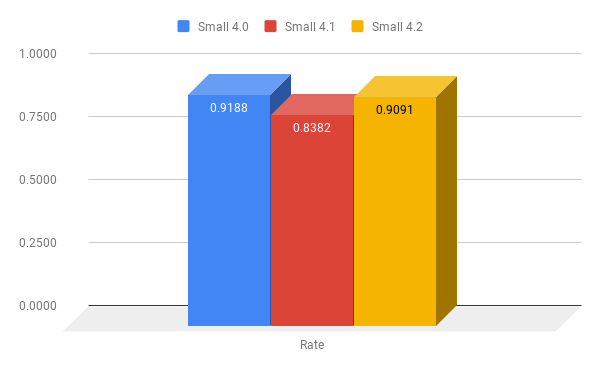
\includegraphics[scale=.7]{charts/rate}
\item Notes: Small 4.0 is the base neural network for 4.1 and 4.2. The differences are as follows: 
\item 4.0 vs 4.1: 4.1 increased the augmentation from 250 photos per class to 500 photos per class, which is reflected in the increase in overall numbers for 4.1. This was not a positive improvement.
\item 4.1 vs 4.2: 4.2 retained the same model as 4.1 and 4.0. 4.2 Used a augmentation size of 300 as well as removed the horizontal flip option from the augmentation. I did this as I thought that flipping a d or b horizontally could lead to classification issues. It does not seem that this had a positive effect. 
\item I also compiled some useful data regarding to the medium (19 class) set.
\item The following is a graph showing the total number of samples vs correct guesses that was achieved during a test on the 7th iteration of the medium set model.
\item 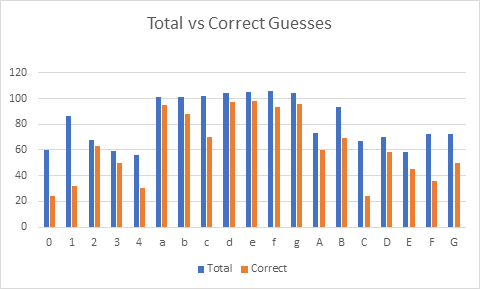
\includegraphics{charts/total-vs-correct}
\item The following graphic used the previous graphs data to find the relationship between sample sizes and correctness.
\item 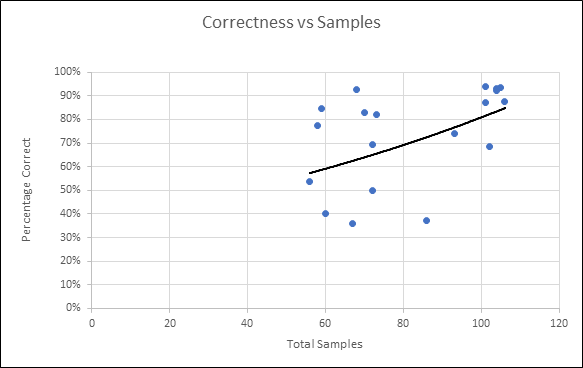
\includegraphics {charts/correct-vs-samples}
\item Given the conclusions of the tests as well as plotting the information into graphs, the model needs more data. The previous chart's trendline clearly suggests that there is a positive relationship between samples taken and the model's success. Although this seems obvious, it was important to isolate each character, as well as rule out the interaction of certain characters. I.e. it was important to figure out if 'b' and 'd' interacted, or if they had high success despite their similarity.
\end{enumerate}

\end{document}
